\documentclass[9pt,technote]{IEEEtran}

%\IEEEoverridecommandlockouts
% The preceding line is only needed to identify funding in the first footnote. If that is unneeded, please comment it out.

\usepackage{cite}
\usepackage{amsmath,amssymb,amsfonts}
\usepackage{algorithmic}
\usepackage{graphicx}
\usepackage{textcomp}
\usepackage{xcolor}

\begin{document}

\title{Statistics for Data Analysis Final Assignment}
\author{Peter Nolan PGDDA (x22154116@student.ncirl.ie)}

\section{Introduction}

\textit{R} was implemented using \textit{RStudio 2022.12.0+353} on MacOS.  The analysis was also done in parallel using a Jupyter notebook in the cloud hosted on the Google Colab service using an $R$ core; this preserves the results of analysis without having to run it.  A GitHub repository also holds the code and the analysis files, which can be downloaded or, for the Jupyter notebook, run in place, via Google Colab, at \texttt{https://github.com/dpnolan/taba}.  

\section{Irish Airport Departures Data}

\begin{figure*}
    \centering
    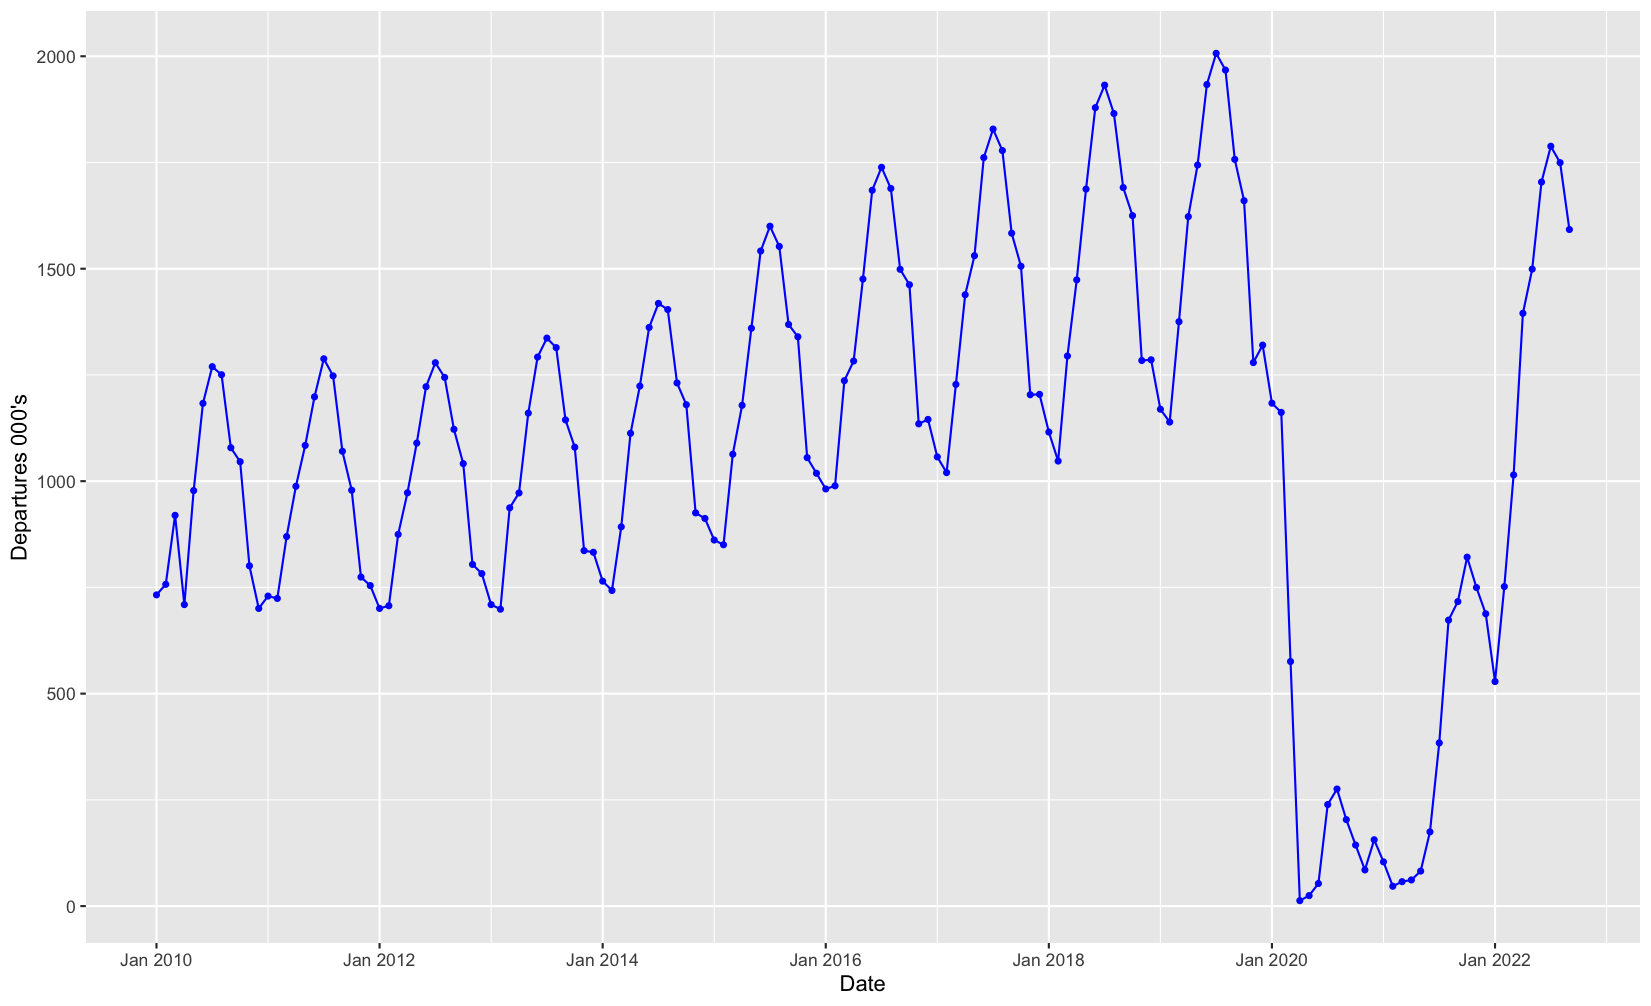
\includegraphics[width=1\textwidth]{ts_departs.png}
    \caption{Departures from Irish airports by month}
    \label{fig:ts_departs}
\end{figure*}

In this section, I estimate and analyse time series models based on monthly observations of departures from Irish airports.  The time series data itself is the only input into this analysis.  No explanation in other variables is available from the data set given and the models I use do not look for one, instead looking to capture and then to understand the other

Data was downloaded in the file named \textit{Departure.csv}.  The file has 153 observations of the numbers in every calendar month of passengers departing from all Irish airports, reported in thousands.  

A simple graph of the departures against dates in figure~\ref{fig:ts_departs} gives a visual summary behaviour that we should aim to understand and forecast. In later sections, I use different time series tools to test, model and forecast these numbers and attempt to evaluate how they can be used in practise.  

\subsection{Data Pre-processing}

To begin with, I manually checked that the dataset had one observation for every single month from and including January 2010 to and including September 2022.  No NA or otherwise unreadable observations or any unsuitable for numerical analysis were found in a visual inspection of this data. 

To allow processing with the specialist R libraries for time series, I transformed the data into a \textit{ts} object defined in the library \textit{tseries}.  Apart from the observations, the start and end dates were included in the definition, along with their frequency of 12, meaning monthly.  

%\begin{figure}[htbp]
%\centerline{\includegraphics[scale=0.2]{density2.png}}
%\caption{Histogram and density function of departures}
%\label{fig:density2}
%\end{figure}

Patterns in the data are visible that we can use to understand and then to forecast the time series.  Four aspects in particular present us with choices in the modelling:

\subsection{Seasonality}Seasonality is clearly visible in the time series and the same pattern consistently shows in all years with the summer holiday months of June, July and August showing the highest passenger numbers in each year, another peak at the Christmas and New Year holidays, then with January and February consistently the lowest.  Figure~\ref{fig:ggseason} shows the seasonality in each year in the full dataset.  Figure ~\ref{monthplot} shows the variation, with bars at the means, across the whole dataset bucketed by month.  

For making decisions involving airport operations such as staffing, buying fuel or flight scheduling, this behaviour is likely to be always relevant.  

\begin{figure}[htbp]
\centerline{\includegraphics[scale=0.2]{ggseason.png}}
\caption{Observations by Year, full dataset}
\label{fig:ggseason}
\end{figure}

\begin{figure}[htbp]
\centerline{\includegraphics[scale=0.2]{monthplot.png}}
\caption{Observations over the full dataset, per month}
\label{fig:monthplot}
\end{figure}

\subsection{Trend and Cyclical Factors} Departures appear level from 2010 to 2013.  However, from 2013 to 2020 the chart shows a pronounced growth trend: Minimum and maximum numbers increase every year, reaching the peak value in the dataset of over two million in July 2019.  The growth happened at the same time as economic growth and increased population in Ireland after the Europe-wide economic crisis early in the decade.  Operating on a longer-term than the seasonality within the year, this behaviour would be important for longer term decision making such as building terminals and buying planes.  

\subsection{Pandemic Shock}

COVID19 impacts are clear to see in the data in the first quarter of 2020, as the disease spread from China to Europe.  By April 2020, traffic at Heathrow airport in London was down by 97\% and some 2.7 billion workers, 81\% of the global workforce were under some form of lockdown \cite{tooze21}.  The economic fallout from the pandemic were all apparent when the departures numbers had a rapid fall in Q1 of 2020 to their low point in this dataset in April 2020 of only 12,800.  

Shocks like this to air travel are much rarer, probably unique since the global influenza pandemic of 1918.  Pandemic insurance was offered by a few insurers, but demand was very low and not part of regular operations planning for almost all businesses\cite{ratliff20}. For our model, this may not be something which can be incorporated easily. Certainly, no similar shock is covered in textbooks on time series \cite{fpp2}.  This would likely be something that the CEO or CFO might take responsibility for given the importance to an airline or airport's relationship with its bank lenders, shareholders and government in such a crisis.  

\subsection{Recovery}

Post-pandemic recovery seems to have seen further differences from both the crisis period of the first few months of 2020, which saw the lowest value in the time series with 12,800 departures in April.  The remainder of 2020 showed departures remaining well below previous values, but seasonality being maintained peaking in the summer months as before, but reaching a maximum level for the year at only 275,500 in August.  

From that low base, 2021 saw a partial recovery back to about half 2019 numbers by the autumn, peaking at 821,000 departures in October compared to 1,660,000 in October 2019.  Starting from a lower point than before, 2022 shows an annual maximum in the summer months of some 1,788,200, close to the highest observations recorded in 2016 and 2017.  This has coincided with the economic rebound, as money saved during the pandemic is spent, and with travel restrictions lifting.  To me, this points towards the effect of the pandemic largely fading away and the regular seaonality and cyclical behaviour returning instead.  

\subsection{Descriptive Statistics}

Descriptive statistics were calculated.  The median and mean departures per month were 1,134,900 and 1,088,600 travellers per month.  Skewness was estimated for all observations at around -0.43, so leading to the right and kurtosis as 2.89, so with the central peak and tails close to, although not matching, those of the normal distribution, as shown in the histogram in the R notebook.  

The observations were grouped by calendar year and a box plot generated for each, as shown in figure~\ref{fig:boxplot2}.  This illustrates the statis from 2010, then the upward trend 2013--2019 and the discontinuity and possible non-stationarity between 2019, before the pandemic, the impact of the pandemic in 2020, and then the strong recovery in departures in 2021 and 2022.    

\begin{figure}[htbp]
\centerline{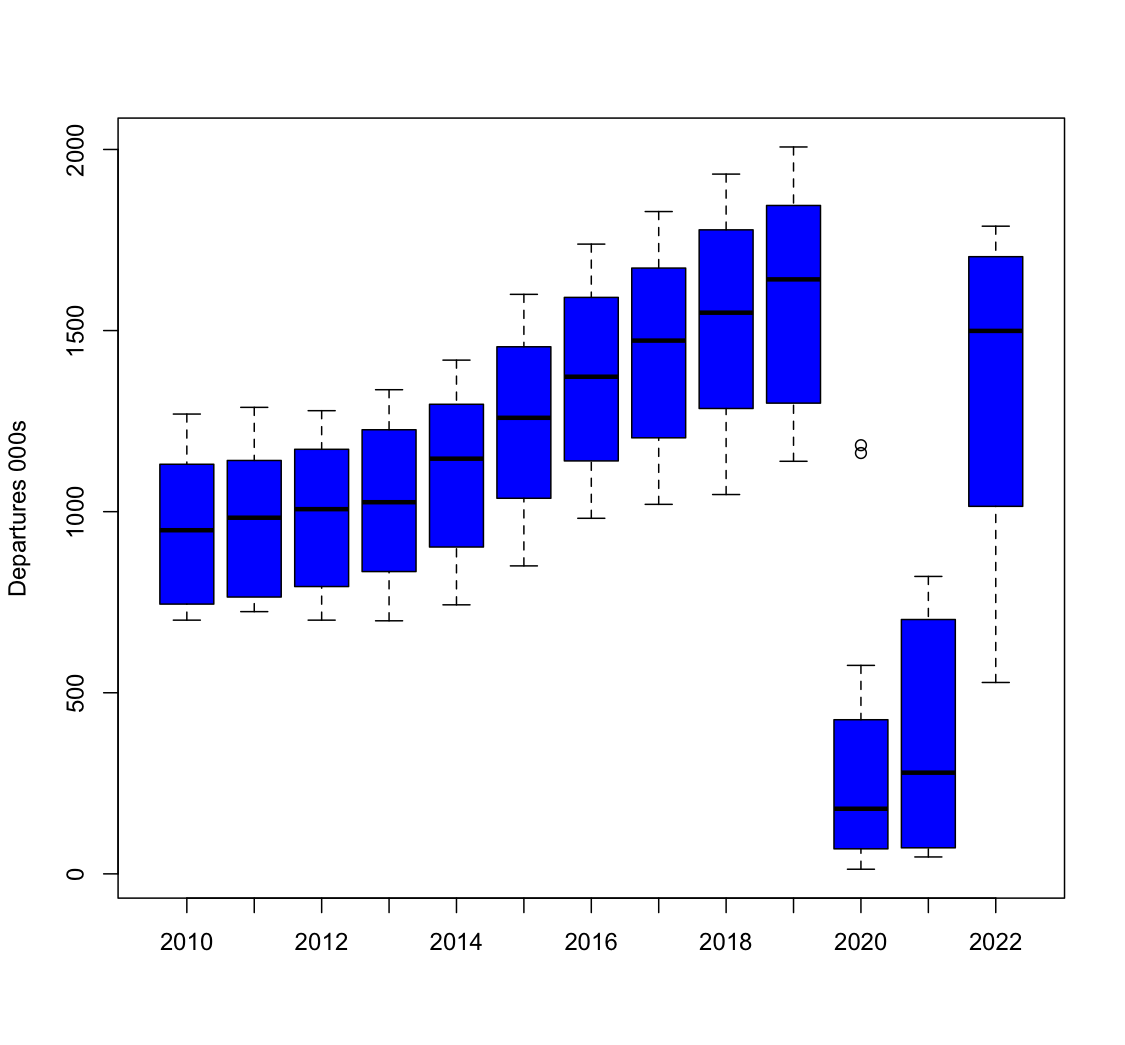
\includegraphics[scale=0.2]{boxplot2.png}}
\caption{Departures by year}
\label{fig:boxplot2}
\end{figure}

A number of t-tests were performed on these sub-samples.  One rejected the two-sided null-hypothesis of equality between the mean of departures for calendar 2013 and 2019 with p.value of $7.7 \ times 10^{-5}$. A second t-test also rejected equality of means for 2019 and 2020, the year of the pandemic crisis.  A third rejected mean equality for the means for 2020 and 2022, what looks to be a second year of the recovery.  All results reinforce the idea that we face four distinct periods in our time-series sample data.  

\section{Estimating an Exponential Smoothing Model}
\label{sec:exp}

Common solutions for forecasting are either exponential smoothing models that I cover in this section or ARIMA models that I discuss below in the next section~\ref{sec:arima}.  The treatment here closely follows \cite{fpp2} chapter 7.  

Given that our visualisation of the time series shows a what is likely to be a trend and seasonality, a sensible starting point is an exponential smoothing model that combines both these with a random element, namely the Holt-Winter (hereafter `HW') model in its additive form i.e. from \cite{fpp2}, section 7.3: 

\begin{equation}
\hat{y}_{t+h|t}=\ell_{t} + hb_{t} + s_{t+h-m(k+1)}
\end{equation}

\begin{equation}
\label{eq2}
\ell_{t} = \alpha(y_t - s_{t-m}) + (1-\alpha)(\ell_{t-1} + b_{t-1})
\end{equation}

\begin{equation}
\label{eq3}
b_t = \beta^{*} (\ell_t - \ell_{t-1}) + (1-\beta^{*})b_{t-1}
\end{equation}

\begin{equation}
\label{eq4}
s_t = \gamma(y_t - \ell_{t-1} - b_{t-1}) + (1-\gamma)s_{t-m}
\end{equation}


Here $\alpha$ is the smoothing parameter for the level, $\beta$ for the trend and $\gamma$ for the seasonal adjustment component.  $\ell_t$ is the smoothed series at $t$, $y_t$ the raw observed value of the series at $t$, h the number of periods ahead we are forecasting for, $b_t$ the estimated trend component at $t$.  

Equation~\ref{eq2} for the level shows a weighted average of a seasonally-adjusted observation in the first part and a non-seasonal component forecast as at $t$.  

Equation~\ref{eq3} for the trend shows how the current estimate of the trend $b_t$ is specified as a weighted average of the change in the smoothed series and the last value of the trend component.  

The seasonal equation~\ref{eq4} shows an average weighted by $\gamma$ between the current seasonal index component and the seasonal index of the same season $m$ time periods ago.

A damping parameter $\phi$ was included in the model by default, to prevent unlimited growth in the trend component. 

With ETS, solutions are estimated so as to minimise the sum of squared residuals of the model.  

\subsection{Estimation}

The ETS function from the \textit{forecast} library was run, with the \textit{model = `ZZZ'} option allowing the software to automatically select the type, whether additive or multiplicative, for the error term, the trend and the seasonality components respectively.   The system estimated an additive model \textit{departs\_fit1} for error, trend and seasonality terms rather than a multiplicative model.  This was in line with prior expectations, as the graphical representation of the time series shows no noticeable increase in variance in the years before the arrival of the pandemic.  

The model \textit{departs\_fit1} scores an AIC corrected for small sample bias, the AICc, of 2,235.89 and Root Mean Squared Error (RMSE) of 105.35.  The smoothing parameters were $\alpha = 0.9999$, $\beta = 0.1413$ and $\gamma = 1 \times 10^{-4}$.  A damping component was estimated with $\phi = 0.8$.  The same parameter estimates and scores came from running the ETS function with the same inputs but with the model explicitly set as additive for all components i.e. `AAA' in \textit{departs\_fit2}.  Figure~\ref{fig:ETSdecomp} shows the decomposition of the full time series observations into the level, trend and seasonality components estimated for \textit{departs\_fit1}.  

\begin{figure}[htbp]
\centerline{\includegraphics[scale=0.25]{ETSdecompfit1.png}}
\caption{Decomposition by ETS additive exponential smoothing on training data}
\label{fig:ETSdecomp}
\end{figure}

A third model without a damping parameter was also run, \textit{departs\_fit3}.  This generated worse scores than the earlier \textit{departs\_fit1} model, with AICc of 2245 compared to 2235 and RSME at 109.567 instead of 105.35.  

\subsection{Forecasts}

Forecasts were generated for 8 months past the end of the dataset.  The model \textit{departs\_fit1} with a damping parameter for the trend specified generated a range of forecasts of 746.3 to 2331.54 with a point forecast of 1538.9.  The model \textit{departs\_fit3} with the same setup except for no dampening, shows a much higher point forecast 1904.69 and a wider dispersion of 941.48 to 2867.9.  

\subsection{Diagnosis}

Running the \textit{forecast::checkresiduals} function on \textit{departs\_fit1} shows a statistically significant autocorrelation of current against values with lag of 1.  The ACF, plotted in figure~\ref{fig:ETSresiduals} also shows significant correlations around 23 and 24 months. A Box-Ljung test reinforces this by rejecting the null hypothesis of no autocorrelation with a p-value of 0.0001575.  A Jarque-Bera test rejects normality also, with a p-value of $2.2 \times 10^{-16}$. 

All this points to information not captured by the chosen model here still to be captured by some different models instead. 

\begin{figure}[htbp]
\centerline{\includegraphics[scale=0.25]{ETSresiduals.png}}
\caption{Testing residuals and the ACF from our ETS model}
\label{fig:ETSresiduals}
\end{figure}

\section{SARIMA Models}
\label{sec:arima}

In this section, I work to fit a model of the SARIMA (Seasonal Autoregressive Integrated Moving Average) type to the time series data.  While the exponential smoothing models in section~\ref{exp} fit a trend and seasonality measurements, the ARIMA class focuses on identifying and estimating relationships between values of the time series at different times of the Autoregression (AR) or Moving Average (MA) types, after adjusting the series to ensure its stationarity.  The treatment here largely follows \cite{fpp2} chapter 8.  

To begin, we can take first differences of our time series until it is stationary.  The function \textit{ndiffs} from R library \textit{forecast} tests for stationary in the time series, whether its properties depend on the time of observation:  In this case, the tests, using all the three options available, namely a KPSS, Augmented Dickey-Fuller and  Phillips-Perron, return a one, a zero and a one value respectively, so that two are indicating that the time series is stationary and does not need differencing before applying an ARIMA model.  

\begin{figure}[htbp]
\centerline{\includegraphics[scale=0.25]{firstdiffs.png}}
\caption{Plotting training data against its first differences}
\label{fig:firstdiffs}
\end{figure}

Doing the \textit{nsdiffs} test, applying the same logic but at time lags matching the seasonality of every 12th value in the case of our monthly data, returns a value of 1, showing non-stationary between every 12th observation in our series.  Together the two test results indicate that our data can be represented by a model of the form ARIMA(p,0,q)(P,1,Q)[12]. 

We may then continue on to plot the autocorrelation and partial autocorrelation functions of the time series, shown in figure~\ref{fig:Acf} and ~\ref{fig:Pacf}.  

The ACF plot shows the correlation of the time series with its own past values: Here, several lag intervals show statistically significant levels different from zero of correlation with a gradual reduction over time, which points to a model with one or more autoregression terms, showing that previous observations in our time series have an influence on our current observation.  

\begin{figure}[htbp]
\centerline{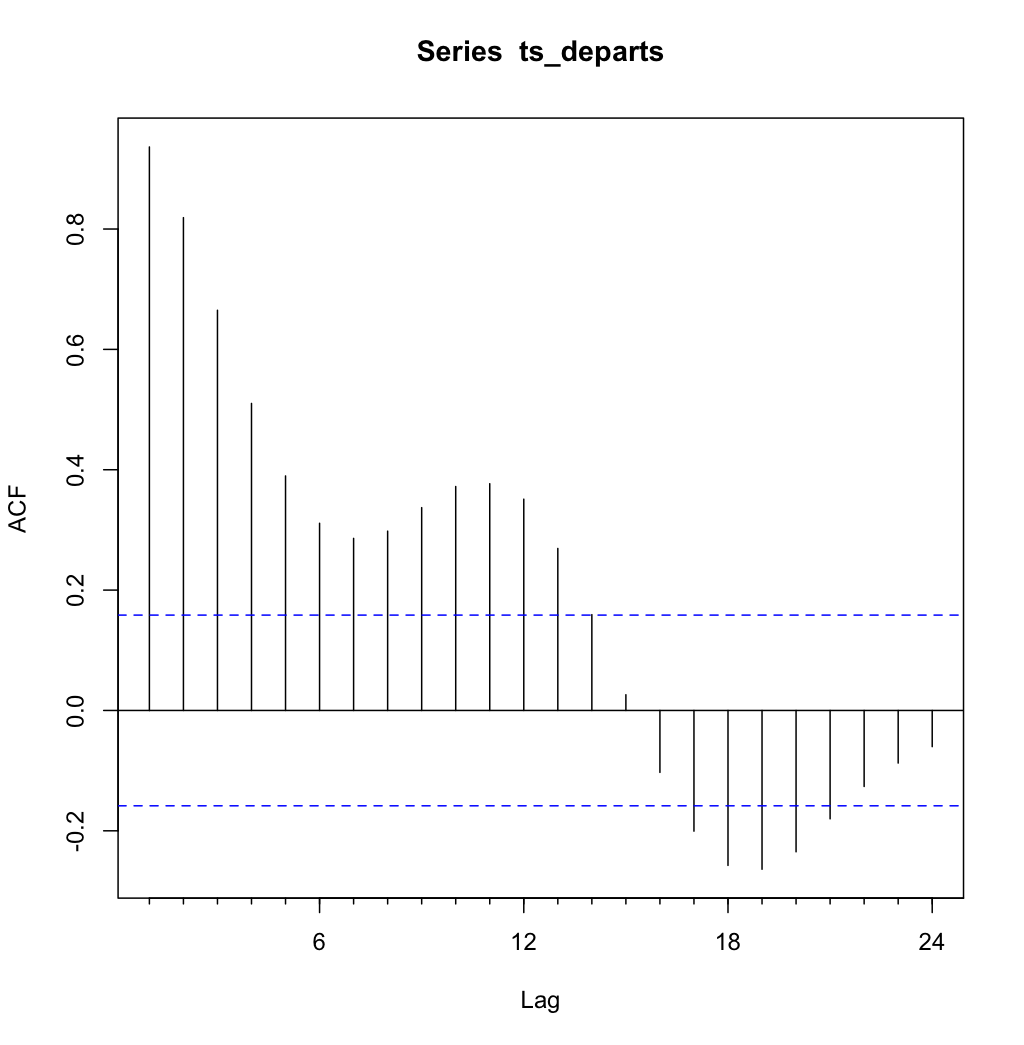
\includegraphics[scale=0.25]{Acf.png}}
\caption{ACF plot}
\label{fig:Acf}
\end{figure}

The PACF graph shows the correlation between the time series and values at each time lag not explained by any lower order autocorrelations.  The large and statistically significant partial autocorrelations at the lags of 1, 2, 3 and 5 are visible the PACF may indicate autoregression at those lags.  The significant autocorrelations at lags of 12 and above may indicate AR or MA processes among the same months' values from different years also.  

\begin{figure}[htbp]
\centerline{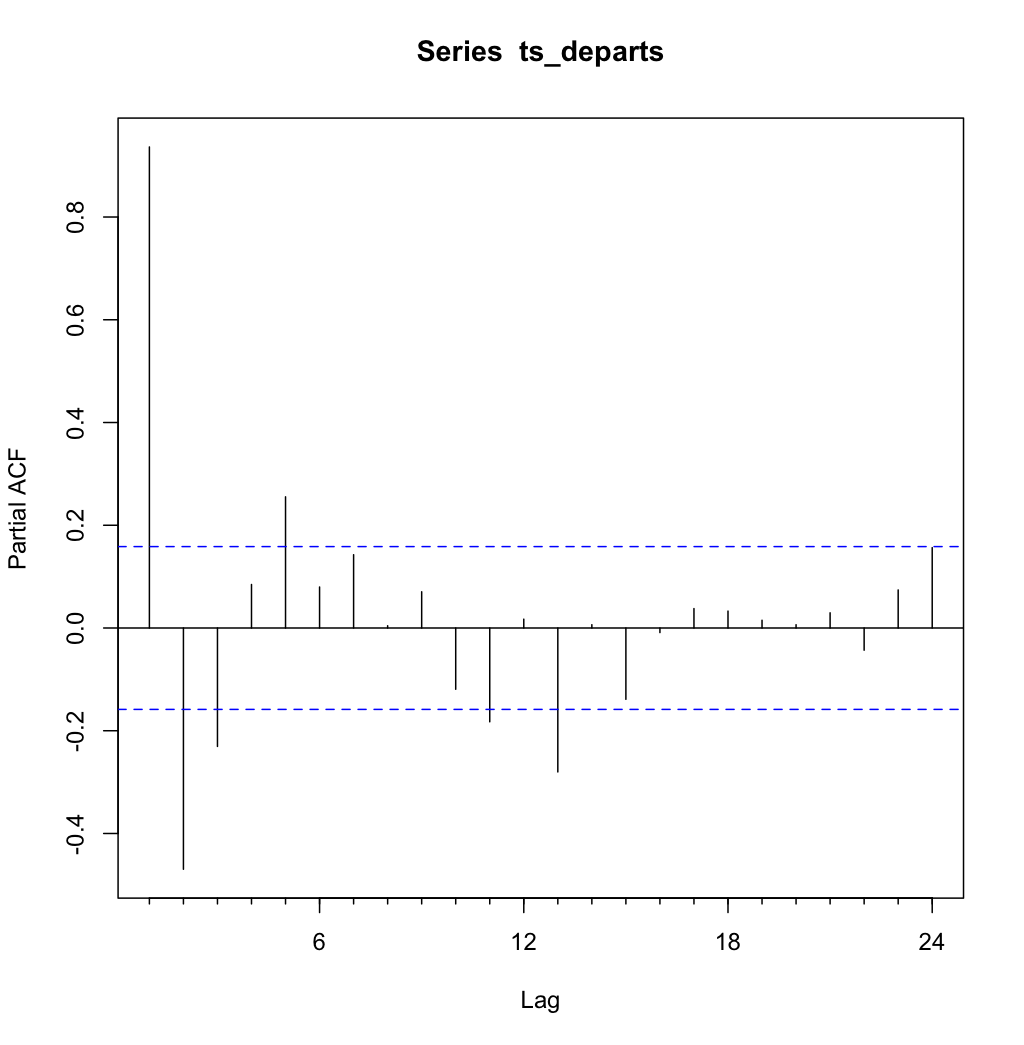
\includegraphics[scale=0.25]{Pacf.png}}
\caption{PACF plot}
\label{fig:Pacf}
\end{figure}

Proceeding to test and select from a number of possible SARIMA models, we may use the \textit{auto.arima} function, again from the \textit{forecast} library, for an automated search.  Given the large number of possible model specifications, searches for the best fit as determined by the AICc score, with the stepwise flag set to FALSE to specify the an exhaustive search and \textit{start.p} and \textit{start.q} both equal to 1 so as to search for the most models possible.  This returns a model specification \textit{sax} of ARIMA(2,0,0)(0,1,1)[12] as being the highest scoring, with RMSE 102.1331, AIC 1742.81 and AICc=1743.1.  Afte I manually specified alternative more SARIMA models of different orders, estimated and scored those, the first model, \textit{sax} remains the best performing candidate.  

Looking at the residuals with the \textit{checkresiduals} function, we can test if the errors left after applying our SARIMA model to the time series show any systematic structure not captured by the model.  The plot is shown in figure~\ref{fig:SARIMA_residuals} and the lack of any statistically-significant autocorrelations would support our hope that the residuals behave like white noise. 

\begin{figure}[htbp]
\centerline{\includegraphics[scale=0.25]{SARIMA_residuals2.png}}
\caption{Testing residuals from our SARIMA model}
\label{fig:SARIMA_residuals}
\end{figure}

Running a Ljung-Box test, the null hypothesis of independence among the residuals is also upheld when tested at lags from 1 to 14, again supporting the view that no autocorrelation and hence no systematic predictability remains within the residuals to capture in an updated version of our model.  

% Plotting the data
% Transform the data if necessary to stabilise the variance
% Check residuals by plotting their ACF and do a Box Ljung test
% Once residuals look like white noise, calculate the forcast values

\subsection{Forecasting}

Our SARIMA model \textit{sax} forecasts 8 months ahead a pattern showing 2023 with the same maximum and minimum levels and seasonality behaviour as in 2016.   This is probably realistic, given the continuing seasonality we see and a continuing re recover from the pandemic's economic effects. The 95\% confidence interval goes from 439 to 2363, a very wide range for uncertainty.  

\section{Simple Time Series Models}

\subsection{Simple Forecasting Benchmark Models}

The simplest of forecasting models are quick to estimate and re-run and conceptually simple.  Most often, these would be used as benchmarks against which to measure any other model proposed and evaluate whether the extra cost and complexlity are justified by the difference in performance.  Also, there may be a theoretical justification, if we hypothesise that our dataset is generated by a model already specified that matches the benchmark.  One important case in finance is the Efficient Market Hypothesis (EMH), the theory that stock prices at any time already reflect all available information \cite{fama1965b}: The naive model implementing a random walk \textit{rwf()} in \textit{R}, is usually the first benchmark to any forecasting model in this domain.  

Following the approach in \cite{fpp2} chapter 6.2 I evaluated four such simple models estimated with the training data.  Their output is plotted in figure~\ref{fig:SimpleModels}. Overall, the bias and variance of these estimators and the RMSE is not good and there seems no strong justification to use them past the H1 2021 test period.  
\begin{itemize}
\item
\textit{mean} which sets the forecast for the test period equal to a constant, the mean of the historical data input, the full training period Jan 2010 to Dec 2020.   the forecast had very high errors, averaging over a million more forecast than realised per month in the test period of Jan 2021 to June 2021: This bias was very large, while variance of the (constant) forecast was zero and the RMSE 423.65.  The high forecast will look better as recovery continues in 2021 and 2022.  However, it has no seasonality and no trend, which are visible in the later data as conditions return to normal.  
\item
\textit{naive} setting the forecast equal to the last observed value of the training data in Dec 2020.  This matched our data quite closely at the nadir of the pandemic: mean error was -68.28, RMSE was 159.53.  However,out of sample performance of the constant forecast of 156 will be very poor during recovery in 2021 and 2022.  The forecast also has no seasonality and no trend, which appear again as conditions return to normal.    
\item
\textit{seasonal naive} the forecast is equal to the last value in the last matching seasonal period, months in our case.  The model gives us a forecast of a bizarre downward shift in early 2021, high forecast errors around 414 and enormous standard deviation of 571, so very high estimator variance. 
\item
\textit{trend} extrapolating by the average change over the training data to estimate the future values. Low estimates from the model are not too bad as forecasts for H1 2021 and bias, with an average forecast error of -52 a month, is comparatively small.  However, this is still in the nadir of the pandemic.  The drift model is not signalling the recovery: In fact, the downward trend on drift is moving in the opposite direction to the recovery's upward trend.
\item
\end{itemize}

\begin{figure}[htbp]
\centerline{\includegraphics[scale=0.2]{SimpleModels.png}}
\caption{Forecasts from the simple time-series models}
\label{fig:SimpleModels}
\end{figure}

\subsection{Time Series Decomposition}

Some simple time series decompositions were also estimated for our training data, splitting out the time series into trend, seasonal and residual components.  The split is plotted in figures~\ref{fig:DecompAdd} and ~\ref{fig:DecompMult}

Additive seems the more suitable as a match for the training period data,as the variance of the time series measured from seasonal peaks to throughs looks like it remains constant through the training data history.  However, both additive and multiplicative models estimted fail the Box Ljung test for independence of the residuals after the model fitting and also the Jarque-Barra tests for normality of the residuals, pointing towards predictability not captured by these models but perhaps deteactable by some other method.  

Forecasts were generated going 12 months forward from the last available datapoint in the model at June 2010 forward to June 2021, but these were negative values of -571.6, which would be meaningless in our model, as there cannot be a negative passenger departure.  In any case, with the mean forecast error being 659.4, the bias on this model would argue strongly against its use as a forecasting tool.  

\begin{figure}[htbp]
\centerline{\includegraphics[scale=0.2]{decompadd.png}}
\caption{Additive decomposition of the training data}
\label{fig:DecompAdd}
\end{figure}

\begin{figure}[htbp]
\centerline{\includegraphics[scale=0.2]{decompadd.png}}
\caption{Multiplicative decomposition of the training data}
\label{fig:DecompMult}
\end{figure}

\section{Applying a Forecasting Model}

From the above analysis, the performance 

\section{Logistic Regression for Analysing a Bank Marketing Campaign}

In this section, I analyse a dataset estimated over several years from the records of a Portuguese bank of the characteristics of a population of consumers and their interactions with the bank.  I relate this data to the customers decision to purchase or not a bank product by estimating and testing a logistic regression model   

\section{Understanding the Dataset}

The dataset consists of records derived from the dataset used by Moro et al.\cite{moro14}.  The file provided, \textit{Bank.csv} provides 45,211 records each with observations of 17 variables which we can use to analyse the purchase decision.  

Most of these variables are categorical variables, namely \textit{job, marital status, education, default, housing, loan, contact, month, previous outcome}.  Also categorical is\textit{y}, the outcome variable.  These have two or more discrete values, all known, with no numerical meaning or ranking among the different values: All these were converted in \textit{R} to what it calls factor variables.  After the categorical variables were converted into R factor variables and added to the dataset, these were dropped from the dataset.  Day was dropped also.  

The numerical variables namely \textit{age, balance, duration, campaign, pdays, previous} were not transformed for this initial analysis, partly to keep them in their more intuitive original form for easier communication, but also because outliers seem comparatively rare.  

All variables were imported into the dataframe \textit{bank}, which is not updated afterwards, and the cleaned and transformed values were added to the dataframe \textit{bank\_clean}, which includes \textit{y} that will be our dependent variable, which is dropped from the othewise identical dataframe \textit{independent\_variables}.  

Below, I show some graphs and descriptive statistics for the variables in the dataset. The full set are available in the \textit{R} code.  Here, as in \cite{hastie21} figure 4.3, the intention is display visually any signficant difference between the values of these variables between the cases with 'yes' and 'no' outcomes which we can expect to be useful in our model.  Violin plots are used to summarise the the numerical variables across the 'yes' and 'no' populations.  Bar charts show the proportions for the other, categorical variables in the 'yes' and 'no' populations.  Code was adapted for the graphs from \cite{chang19} section 6.8 \& 6.9. 

\subsection{Y} 

\textit{Y} is a categorical variable showing, yes or no, whether the client has subscribed for the deposit product the bank has offered.  This is the dependent variable that we would expect to be able to try to explain using the other independent variables in the dataset.  This binary variable was converted into the R factor variable \textit{y\_factor} with values 'yes' and 'no'.  

One important fact to note immediately is that the observations are split into 39,922 'no' and 5,289 'yes' observations.  So, calculating 5289/(39922+5289)=  0.1169848, we see that approximately = 11.7\% of the observations are for 'yes' cases.  This is close to the 12.37\% rate of success in the original study\cite{moro14}.  As Moro et al. observe, this means that the dataset is unbalanced between the 'yes' and 'no' cases.  A naive estimator with no logic that just predicts 'no' in every case will still be correct about 88.3\% of the time.   This is not uncommon but requires adaptations in our model training and interpretation, described in detail in section~\ref{sec:imbalance} below.  

\subsection{Days Since Last Contact}

The variable \textit{pdays} records the number of days since last contact with the customer.  Most observations almost 37,000 are equal to -1.  I assumed that these represent no recorded values, so replaced these with NA instead, making this the only variable in the dataset with any NA values.  The other 8,257 observations are positive integers.  

\subsection{Age}

In our violin plot in figure~\ref{fig:graph1age}, we see the distribution of the age variable in two separate buckets for 'yes' and 'no' customers.  The white dot shows the median.  The black area shows the box plot, with top and bottom edges at 75 and 25 percentile levels.  The results show some differences, with higher mean but lower median for 'yes' and significantly more skew and kurtosis for 'yes'.

\begin{figure}[htbp]
\centerline{\includegraphics[scale=0.25]{graph1age.png}}
\caption{Age in yes and no observations}
\label{fig:graph1age}
\end{figure}

\subsection{Balance}

Note that balance, which might usually mean a relationship balance, the total balance summing across all accounts and loan balances across the relationship with the bank, is in the dataset but not in the document.  As it is potentially useful, I include it in the analysis here as a numerical variable.  As shown in our violin plot in figure~\ref{fig:graph3balance}, the 'yes' population has bigger relationshiop balance, with mean 1804 v 1303 EUR and median 733 v 417 EUR. 'yes' population also has far fewer zero or very low balance values than 'no'.  

\begin{figure}[htbp]
\centerline{\includegraphics[scale=0.25]{graph3balance.png}}
\caption{Balance in yes and no observations}
\label{fig:graph3balance}
\end{figure}

\subsection{Duration}

Figure~\ref{fig:graph4duration} shows the duration of the previous contact with the bank; 'yes' has fewer short conversations, a mean 537 seconds (about 9 mins) v 221 (under 4 mins) for 'no', median value of 426 v 164 i.e. 7 minutes compared with 2.5 minutes.  

\begin{figure}[htbp]
\centerline{\includegraphics[scale=0.25]{graph4duration.png}}
\caption{Duration in yes and no observations}
\label{fig:graph4duration}
\end{figure}

\subsection{Campaign}

The 'yes' population has lower number of contacts made by the bank during this campaign, mean - 2.14 v 2.85.  The distribution is shown in figure ~\ref{fig:graph5campaign}.

\begin{figure}[htbp]
%\centerline{\includegraphics[scale=0.25]{graph5campaign.png}}
\centerline{\includegraphics[scale=0.2]{graph5campaign.png}}
\caption{Campaign in yes and no observations}
\label{fig:graph5campaign}
\end{figure}

\subsection{Previous}

The 'yes' population saw more contacts before this campaign, 1.17 v 0.5, but the median for both subsets is zero contacts before this campaign, so this variable may not have much predictive power. The graph is shown in figure~\ref{fig:graph6previous}.  

\begin{figure}[htbp]
\centerline{\includegraphics[scale=0.2]{graph6previous.png}}
\caption{Previous in yes and no observations}
\label{fig:graph6previous}
\end{figure}

\subsection{Month and Day}

Since the original dataset has observations from over five years of data 2008--2013, the date variables for the last contact offer the potential for finding seasonality in the data.  For the month, we might expect to see seasonal effects, with consumers spending most during summer holidays and the Christmas period.   These periods may be drawdowns of saving rather than new saving, so to 'no' in our caes here and lead instead to savings through the bank's offering at other times of the year.  The month was converted to a factor variable and retained for our model.  

The distributions of observations by month for both the 'yes' and the 'no' populations are shown in 
figure~\ref{fig:graph7month}.  In the 'yes' population, Feb, Mar, Apr, Oct appear as a bigger proportion than in 'no'.  May is also much bigger in the 'no' population.  This points to predictive power in the month variables.  

\begin{figure}[htbp]
\centerline{\includegraphics[scale=0.25]{graph7month.png}}
\caption{Months in yes and no observations}
\label{fig:graph7month}
\end{figure}

For the day of the month, there are many values for a calendar day from 1 to 31, which could make for a lot of extra categorical variables.  Also, these numbers may be for different days of the week in different months and years.  Without more date data, the day was considered as likely to be irrelevant and not brought into the model.   

\subsection{Job}

Figure~\ref{fig:graph8job} shows the breakdown of job categories by 'yes' and 'no' population.  We can notice that the 'yes' population has a lower proportion of blue-collar, more retirees and some more students.   

\begin{figure}[htbp]
\centerline{\includegraphics[scale=0.25]{graph8job.png}}
\caption{Job category in yes and no observations}
\label{fig:graph8job}
\end{figure}

\subsection{Other Characteristics}

More people who are single and have third-level education appear to have subscribed in the past, shown in figure~\ref{fig:graph9and10}.  

\begin{figure}[htbp]
\centerline{\includegraphics[scale=0.25]{graph9and10.png}}
\caption{Marital status and education in yes and no observations}
\label{fig:graph9and10}
\end{figure}

The default variable was assumed to be an indicator of a past credit default event by the customer.  It seems to account for very few observations, but at a lower proportion among the 'yes' population.  

Many fewer people with mortgages appear to have subscribed in the past (figure~\ref{fig:graph11and12}).  They may be directing surplus cash to paying down the housing debt rather than extra deposit accounts.  

\begin{figure}[htbp]
\centerline{\includegraphics[scale=0.25]{graph11and12.png}}
\caption{Has a past default event and has mortgage in yes and no observations}
\label{fig:graph11and12}
\end{figure}

\begin{figure}[htbp]
\centerline{\includegraphics[scale=0.25]{graph13and14.png}}
\caption{Has personal loan and contact method in yes and no observations}
\label{fig:graph13and14}
\end{figure}

Previous outcomes, the customer having responded favourably ('success') to past marketing campaigns shows a visible difference between the 'no' and 'yes' populations in figure~\ref{fig:graph15poutcome}.  This may be a promising variable for use in prediction.  

\begin{figure}[htbp]
\centerline{\includegraphics[scale=0.25]{graph15poutcome.png}}
\caption{Previous decision to buy in yes and no observations}
\label{fig:graph15poutcome}
\end{figure}

\section{Building a Logistic Regression Model}

The objective of our modelling is estimate a binary logistic regression model to predict, using variable observations in the record, the decision to subscribe (\textit{y}) or not to the deposit product.  

Without detailed date data, this is a cross-sectional analysis with a focus on explanation rather than a time-series model.  The objective is also, unlike in our time-series models above, a numerical forecast, but rather a classification analysis, forecasting the binary outcome - to buy or not buy, 'yes' or 'no'.  

Above, I have argued for including 16 of the 17 likely independent variables available, dropping 'Date' only.  As a first pass model, I also wish to avoid any dimension reduction techniques for now, so as to cover the full spectrum of available and potentially useful variables in full detail.  As this is a first exploration and as there is no theoretical model we are estimating, focusing on parsimony in the model risks dropping valuable information before it is understood: The modelling process is as useful in the long term as a learning process for the modeller as it is a rigorous proof.  Neither can the nine factor variables be easily included in this.  

\subsection{Estimating the Full Model}

To begin with, a logistic regression model named \textit{glm.all} was estimated in \textit{R}, following the process in James et al. \cite{hastie21} \S 4.7.2.  This used  all the candidate variables but for the \textit{pdays} in the dataset.  

The linear regression model assumes a linear relationship between the probability of the dependent variable and the values of the independent variables i.e.
\begin{equation}
P(Y_i) = \frac{1}{\beta_0 + \beta_1 X_1 + \dots +\beta_n X_n}
\end{equation}

Using maximum liklihood (ML) estimation, we chose the values of the $\beta_i$ that fit most closely with the observed data, minimising the log-likelihood function.  Deviance is calculated as $-2 \ times log-likelihood$
Null deviance on estimating \textit{glm.all} was 32631 on 45210  degrees of freedom, compared with the residual deviance, that remaining unexplained portion after estimating our model, was 21,578 on 45170 degrees of freedom.  An AIC statistic of of 21,660 was returned.  

The model output Wald statistics and associated probabilities for the 42 coefficient estimates show that, at a 5\% two-sided level of significance, all the variables were assessed as significant except for 7, namely \textit{age} and \textit{previous}, the categories \textit{job} as \textit{unknown} or \textit{unemployed}, \textit{marital} equal to \textit{single} and \textit{default} as \textit{yes}, \textit{contact} as \textit{telephone} or \textit{other}, or \textit{poutcome} equals \textit{unknown}. 

To test the fitted model, we estimated some of the pseudo-$R^2$ models that can give some idea of the explanatory power of the model.  The Cox Snell and Nagelkerke $R^2$ were estimated by \textit{R} as 21.687\% and 42.19\%, so indicating some explanatory power for the model.  The Hosmer-Lemeshow statistic returned a probability value of zero, indicating that the fitted model did not show statistically significant differences from the null hypothesis of zero coefficients.   

\subsection{Model Selection}

Adding back the \textit{pdays} variable that we had left out when estimating \textit{glm.all} above and estimating the model with the extra variable (\textit{glm.all2})leads to no improvement.  The coefficient for pdays has a probability value of 14.95\%, far from significant.  Many other variables also come up as insignificant also.  

Null deviance was 8919.8 on 8256  degrees of freedom, residual deviance 5809.6 on 8215 degrees of freedom, much lower than with \textit{glm.all}, as some 36,954 observations deleted due to the NA values in the \textit{pday} field, most of the records in the dataset.  All this points to dropping the \textit{pdays} variable from the model as insignificant.  

\subsubsection{Stepwise model selection}
\label{subsec:step}
We continued to set up an automated stepwise model selection for the logistic regression. Defining one model with no explanatory variables, so only the intercept terms, \textit{null\_model} and one with all the variables in glm.all above as \textit{full\_model}, a search in both directions was specified.  

After iterating, a model \textit{glm\_step\_AIC} dropping the \textit{age} and \textit{default\_factor} ends up generating the lowest AIC, of 21,656, compared to the 21,660 AIC of \textit{glm.all}.  Coefficients are very close for the remaining variables to those on \textit{glm\_step\_AIC}.  

\subsection{Cross-Validation of the Model}
\label{subsec:crossval}

James et al.\cite{hastie21}(5.1) strongly recommend cross-validation, the family of methods that split the dataset between a portion used for estimation and a part held back from the training data, to test how the performance of the estimates generalise on data not seen in training.  This is also a standard technique used in evaluating machine learning models like neural networks and decision trees that are tested in the original analysis of the dataset by Moro et al. \cite{moro14}. 

Using the \texttt{R caret} library and documentation \cite{caretdocs}, I ran a k-fold cross-validation with $k=5$, the dataset split randomly (although in my code with a seed =1 to allow replication) 5 times in sequence and running the estimation and testing of our logistic regression model \textit{glm.all}.  The process was repeated for the model \textit{step\_model} estimated above in ~\ref{subsec:step} which drops the \textit{age} and \textit{default\_factor} independent variables but which had a better fit indicated by lower AIC score.  The coefficients were very close to the ones estimated above and the AIC scores identical.  

 This would likely make us happier to accept the \texttt{glm.all} model as a useful estimator. No method seems to be agreed in the literature for calculating DOF for k-fold cross-validation like this and so no $t$ or $F$ or Wald statistics can be calculated.  Nevertheless, the process is standard in the machine-learning literature and is  `Perhaps the current gold standard method to reliably estimate model performance'\cite{lantz15} (page 343).

\section{Model Performance and Applications}

\subsection{Evaluating the Coefficients}

Our logistic regression model allows us to understand what variables are associated drive the consumers' decision to subscribe or not 

Prioritising among the estimated coefficients $\beta_i$, for \textit{glm.all}, the most important for users are the large, positive and statistically significant values.  Prioritising among the factors, the five largest are those for the months of March, September, October and December and for $poutcome=success$.  Intuitively, this makes sense, that a seasonal effect and a previous subscription all are associated with a positive decision to  

The log odds in the model are calculated as 
\begin{equation}
log\left(\frac{p(X)}{1-p(X)}\right) = \beta_0 + \beta_1 X_1 + \dots +\beta_n X_n
\end{equation}
Taking the exponent of the coefficient gives the odds ratio, in this case $e^{2.299} = 9.97$, so that the odds that a customer who had subscribed during a previous marketing campaign doing so in this campaign would be 9.97 times greater than for another customer who had not.  The obvious implication is that the bank should target these customers to make sales.  

Month factor variables showing interesting odds ratios are March at 15.171, September with 7.256, October 7.79 and Dec 6.18.  The implication is that the bank would also benefit from focusing resources, perhaps marketing expenses through advertising, direct mail, special offers or other interactions targeting customers at these times in the year.  The retired, students and those with third-level education, with log odds $e^{\beta_i}$ of 1.29, 1.47 and 1.46 respectively, also look on the basis of the model to be more likely to be subscribers.  

\subsection{Classification in the Imbalanced Dataset}
\label{sec:imbalance}

Once we have estimated the models, however, how do our models perform in classifying the 'yes' or 'no' customers?      
  
Following the classification logic in James et al. (2021) \cite{hastie21} \S 4.3 and \S 4.7.2.where the probability of a \textit{Y\_factor} over 50\% is classified as a 'yes', the \textit{glm.all} or \textit{step\_model} both would forecast, using our observed dataset, that there would be 42,389 'no' values of \textit{y\_factor}, compared with the observed number in the dataset of 39,922 and 2,822 'yes' values, compared to the actual realised number of 5,289, a severe underestimate of the 'yes' cases.  If we were using the logistic regression models, the sensitivity, our True Positive Rate, only 34.71\% of the true  'yes' records will be correctly identified as such by the model, an unimpressive performance. 
\begin{equation}
\frac{True Positives}{True Positives + False Negatives} = \frac{1836}{1836+3453} = 34.71\%
\end{equation}

A full confusion matrix is shown below in table~\ref{tab1}.  Given the imbalance towards 'no' cases in the dataset, the sensitivity, or True Negative Rate, the portion of the 'no' values successfully predicted by the model, is much higher: 

\begin{equation}
\frac{True Negatives}{True Negatives + False Positives} = \frac{33,597}{33,597+6,325} = 97.535\%
\end{equation}

\begin{table}[htbp]
\begin{center}
\begin{tabular}{|c|c|c|}
\hline
& \textbf{Y\_factor}&\\
\hline
\textbf{Predicted}&{\textbf{No}}&{\textbf{Yes}} \\
\hline
\textbf{No}&{\textbf{38,938}}&{\textbf{3,453}} \\
\hline
\textbf{Yes}&{\textbf{984}}&{\textbf{1,836}} \\
\hline
\end{tabular}
\label{tab1}
\caption{Confusion Matrix with Classification Threshold = 50\%}
\end{center}
\end{table}

Since barely 11.7\% of the observations are 'yes' cases in our dataset, as Moro et al. observe, this means that the dataset is unbalanced between the 'yes' and 'no' cases.  A naive estimator with no logic that just predicts 'no' in every case will still be correct about 88.3\% of the time.  Among the solutions commonly used \cite{branco17}, we could adjust the threshold value for classifying a prediction as a 'yes' from 50\% down to the 11.7\% population value.  The confusion matrix that results is shown below in table~\ref{tab2}.  The Sensitivity then becomes $4384/(4384+905) = 82.9\%$, the Specificity $33597 / (33597 + 6325) = 84.16\%$.  

\begin{table}[htbp]
\begin{center}
\begin{tabular}{|c|c|c|}
\hline
& \textbf{Y\_factor}&\\
\hline
\textbf{Predicted}&{\textbf{No}}&{\textbf{Yes}} \\
\hline
\textbf{No}&{\textbf{38,937}}&{\textbf{905}} \\
\hline
\textbf{Yes}&{\textbf{6,325}}&{\textbf{4,384}} \\
\hline
\end{tabular}
\label{tab2}
\caption{Confusion Matrix with Classification Threshold = 11.7\%}
\end{center}
\end{table}

Alternatively, we could resample the dataset, generating new observations by adding multiple copies of the 'yes' records, which I have done also in the attached \textit{R} script, resulting in very similar sensitivity and specificity as for the reduced threshold case above.  

Following the process in \cite{lantz15}, I then estimated the ROC curve, shown in Figure~\ref{fig:ROC}.  This graphs the trade-off between identifying the 'yes' cases identified by our model, the Sensitivity, the true positives while trying to minimise the number of the false positives for 'no' cases which is (1-Specificity).  

\begin{figure}[htbp]
\centerline{\includegraphics[scale=0.25]{ROC.png}}
\caption{ROC curve for our model with classification threshold of 11.7\%}
\label{fig:ROC}
\end{figure}

\section{Conclusions and Future Work}

Conclusions

Word Count = xxxx, excluding references

\bibliographystyle{IEEEtran}
\bibliography{dpnolan}

\end{document}